%start by defining the document class
\documentclass{article} 

%below the package used for hyperlinking
\usepackage{graphicx}
\usepackage[brazil]{babel}
\usepackage{float}
\graphicspath{ {./images/} }


%Parameters for titles
\title{ Simulação de Sinais Cerebrais de Espectroscopia por 
Ressonância Magnética: Da Criação à Corrupção (Por Ruído)}
\author{João Victor Dell Agli Floriano}
\date{08/10/2024}


%beggining of doc
\begin{document}

%inserting the title defined above
\maketitle

\section{Resumo}
Apesar de o formalismo de Fourier ter representado uma importante revolução na área de processamento 
de sinais, ele apresenta limitações de identificação de sinais específicos em espectros com alto grau 
de superposição de picos. Nesse contexto, o Matrix Pencil Method (MPM) foi apresentado como uma 
alternativa de pós-processamento, visto que sua aplicação permite uma melhor separação das componentes 
de interesse do sinal.  Entretanto, o método ainda carece de limites bem definidos, particularmente no 
que se refere à aplicabilidade específica aos dados de Espectroscopia por Ressonância Magnética (MRS), 
nos quais o nível de ruído pode ser um desafio extra. Com o objetivo de investigar tais limites, foram 
implementadas rotinas para simulação de sinais sintéticos de MRS cerebral. Esses sinais foram então 
corrompidos com ruído de distribuição gaussiana, possibilitando o estudo de como diferentes valores de 
desvio padrão se comportavam nas várias etapas do processo de análise dos mesmos. Os primeiros resultados 
sugerem uma relação aproximadamente linear para valores mais baixos de ruído e uma saturação para valores 
mais altos. Os limites destes comportamentos, bem como sua caracterização para diferentes condições do sinal 
simulado, ainda estão sendo completamente caracterizados.
\section{Introdução}

\begin{enumerate}
    \item Falar do objetivo a curto e longo prazo do presente trabalho.
    \item Falar sobre a importância de se ter um ambiente controlado para o objetivo final do trabalho. 
\end{enumerate}

\section{Métodos}

A fim de atingir o objetivo final de avaliação do MPM em sinais cerebrais de MRS, algumas etapas foram 
necessárias para que as condições ideais de testagem fossem estabelecidas. Para que esse algoritmo 
seja devidamente avaliado, é necessário primeiro garantir um quantidade suficiente de sinais de 
MRS das mais variadas condições para que uma análise estatística adequada seja feita. 

\subsection{Simulação}

Partindo desse objetivo, a primeira etapa do projeto foi a criação de um ambiente de simulação
que tivesse a capacidade de lidar com as demandas do projeto. A simulação, escrita em uma biblioteca 
própria customizada de python, parte da equação básica de modelagem de um sinal de ressonância magnética.

\begin{equation} \label{eq:1}
    M(t) = M_0 e^{i(\omega t + \phi)} e^{\frac{-t}{T_2}}
\end{equation}

A equação \ref{eq:1} descreve a evolução da magnetização transversal medida ao longo do tempo da parte da amostra medida ao longo do tempo, em Unidades Arbitrárias (U.A.). 
Apesar de ter o tempo $t$ como variável principal, ela também depende de mais alguns parâmetros para 
funcionar: $\omega$, que descreve a frequência oscilação do sinal; $\phi$, que define a fase inicial do 
sinal; $T_2$, que define o tempo de decaimento da magnetização transversal. 

Apesar de inicialmente fornecer uma boa modelagem do sinal, essa equação por si só não da conta de simular todo o processo de 
uma aquisição de um sinal de MRI, visto que ela não considera os procedimentos de eco de spin e gradiente de campo. 

Os ecos de spin, detectados pela primeira vez em 1950 por Erwin Hahn \cite{PhysRev.80.580}, ocorrem quando, após se provocar a 
inclinação dos spins por meio de um pulso de $\frac{\pi}{2}$, os mesmos são desviados novamente, agora por um pulso que os desvia em 
$\pi$ radianos no plano perpendicular ao transversal. Esse novo desvio provoca um refaseamento dos spins, de maneira que a intensidade
da magnetização alcance um novo máximo antes de decair novamente, como se todo o processo fosse reiniciado. Esse procedimento é 
essencial nos processos de aquisição de sinal pois permite a redefinição do tempo inicial de captura dos sinal, evitando qualquer erro 
associado ao início do procedimento de excitação dos spins.

Na biblioteca customizada, esse procedimento foi adaptado como sendo um evento que ocorre durante a simulação do sinal, a qual o 
usuário fornece o instante de tempo que é feito o desvio, e o programa provoca o fenômeno adicionando uma fase de $\pi - 2\theta$, 
como demonstrado na figura \ref{fig:1}, sendo $\theta = \omega \Delta t$, e $\Delta t$ a quantidade de tempo a qual o sinal evoluiu 
até a realização do desvio.   

\begin{figure}[H] 
    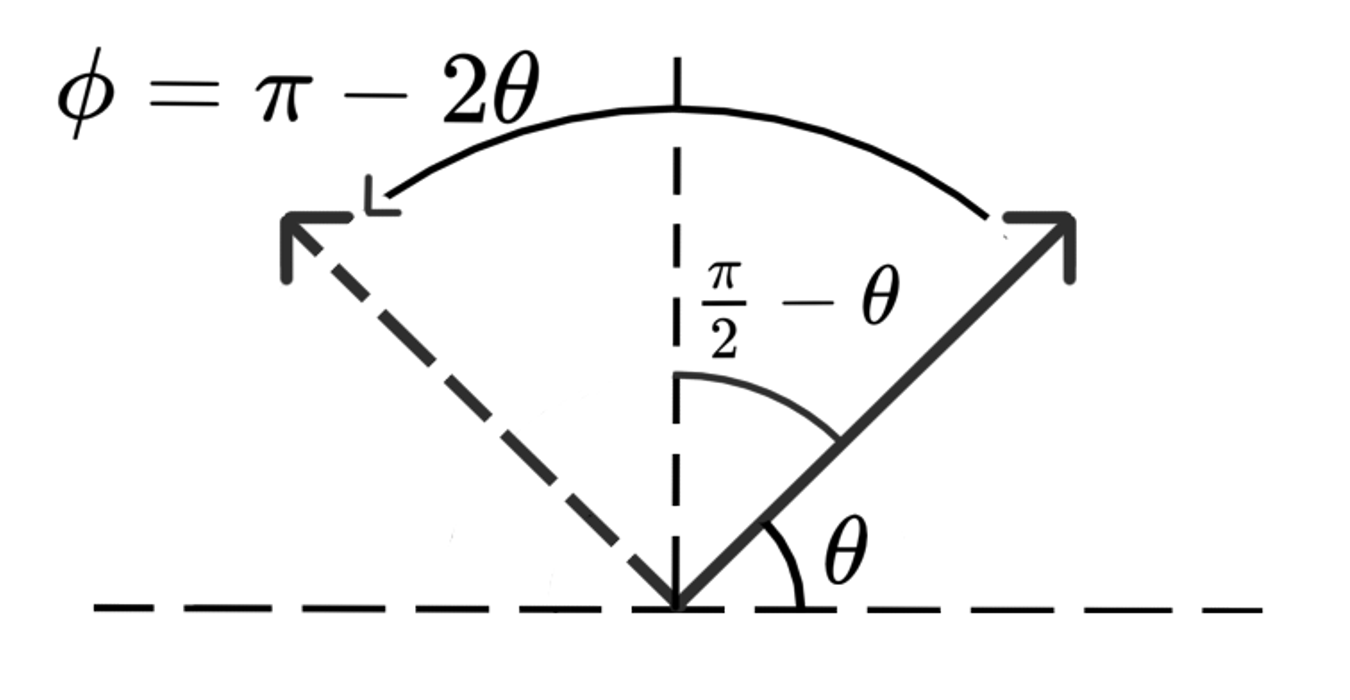
\includegraphics{spin-echo.png}
    \caption{Fase adicional para deslocamento de eco de spin }
    \label{fig:1}
\end{figure}

O gradiente de campo é outro procedimento do processo de aquisição de um sinal de MRI. Apesar de sua principal utilidade ser a 
seleção de uma região de interesse do sinal por meio da indução de uma frequência de ressonância fora da janela de excitação 
nos spins abaixo de um gradiente, a sua implementação nesse programa foi feita para replicar o efeito de ecos de spin 
por uma abordagem diferente. Neste caso, o gradiente já atuante sobre a amostra tem sua direção invertida, o que provoca uma inversão
na direção das frequências de oscilação dos spins, os fazendo seguir na direção contrária. Como se trata de uma fórmula analítica, 
apenas inverter os sinais não é o bastante, pois o sinal se comportará como se tivesse, desde o começo, se movimentado na direção 
contrária. Para corrigir esse problema, uma fase de $2\theta$ deve ser adicionada ao processo após a inversão, como demonstrado pela figura
\ref{fig:2}, sendo $\theta = \omega \Delta t$. Essa fase adicional irá posicionar os spins na posição anterior à inversão, emulando 
uma inversão real.

\begin{figure}[H] 
    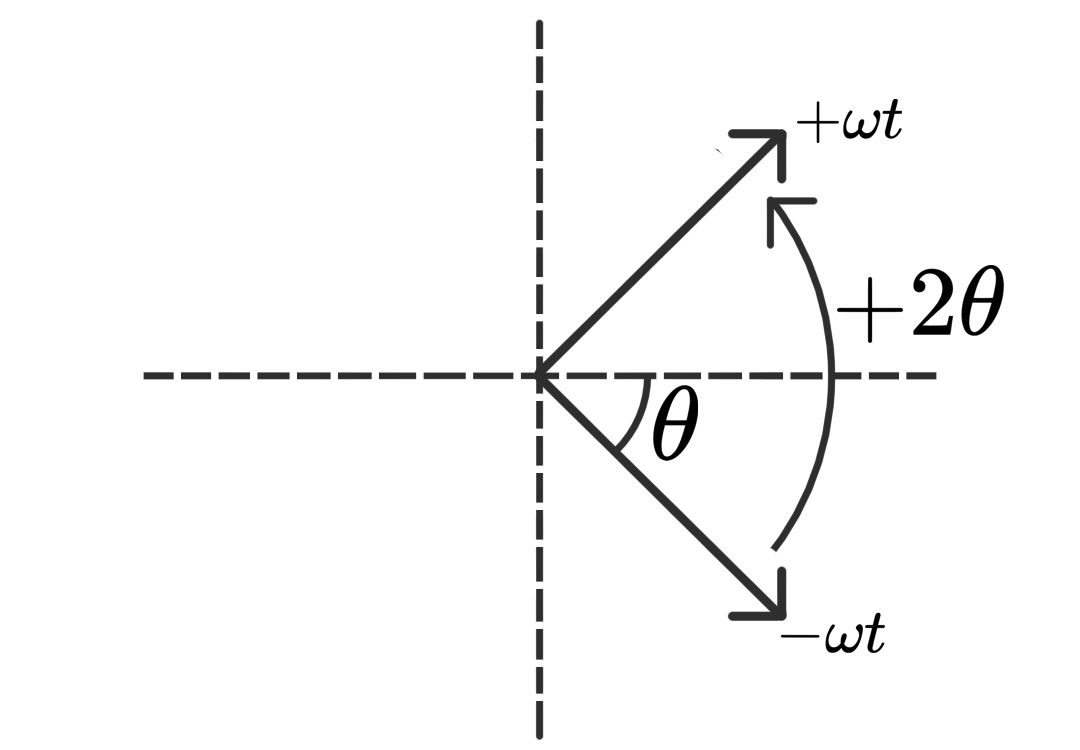
\includegraphics{gradient.png}
    \caption{Fase adicional para a inversão do gradiente}
    \label{fig:2}
\end{figure}

\subsection{Aplicação de Metabólitos}

Com o estabelecimento dos instrumentos necessários para a simulação de sinais de MRS, foi possível então prosseguir para a próxima etapa:
a simulação de sinais cerebrais de MRS.

O procedimento de Espectroscopia por Ressonância Magnética (MRS), apesar de compartilhar dos mesmos procedimentos do MRI, possui objetivos 
diferentes. Enquanto o MRI se preocupa com uma imagem anatômica, ou seja, uma malha de voxels, a MRS se preocupa com a informação contida em apenas um voxel ou grupo 
reduzido de voxels, denominados voxel-of-interest (VOI). O sinal obtido no VOI é analisado suprimindo os efeitos de lipídeos e água, restando 
apenas os sinais de ordem menor, relativos à ruído e a, principalmente, metabólitos. Metabólitos são moléculas orgânicas de forma e composição 
variadas, sendo essenciais em processos celulares. Por, em sua maioria, possuírem átomos de hidrogênio, os mesmos respondem ao sinal de excitação 
de ressonância, fornecendo uma resposta próxima ao sinal esperado, diferindo entre si por uma pequena diferença. Essa diferença, denominada deslocamento químico, 
é causada por efeitos eletrônicos de sua vizinhança química, e é representado na literatura pelo símbolo $\delta$. Seu valor é calculado de maneira 
relativa, dado pela equação \ref{eq:4}, usando o valor de um composto, usualmente o Tetrametilsilano (TMS) \cite{}, como referência.

\begin{equation} \label{eq:4}
    \delta = \frac{\nu _{amostra} - \nu _{ref}}{\nu _{ref}}
\end{equation}


Foram organizados na tabela \ref{table:1}, a partir do trabalho de Danilo Mendes \cite{Silva2020-io}, os parâmetros de desvio químico ($\delta$), tempo de relaxação 
transversal ($T_2$) e amplitude de alguns metabólitos comumente encontrados no cérebro, sob regime de 3T. Esses valores são então usados como entrada na simulação
previamente discutida, para a geração de sinais cerebrais. 

\begin{table}[H] 
    \centering
    \begin{tabular}{|l|c|c|c|}
    \hline
    Metabólito & $\delta$ (ppm) & $T_2$ (s) & Amplitude (U.A.) \\
    \hline
    GABA & 1.9346 & 0.0199 & 0.2917 \\
    NAA & 2.0050 & 0.0735 & 0.4289 \\
    NAAG & 2.1107 & 0.0066 & 0.0290 \\
    Glx2 & 2.1157 & 0.0909 & 0.0184 \\
    GABA2 & 2.2797 & 0.0833 & 0.0451 \\
    Glu & 2.3547 & 0.1163 & 0.0427 \\
    Cr & 3.0360 & 0.0926 & 0.2026 \\
    Cho & 3.2200 & 0.1136 & 0.0776 \\
    M-Ins3 & 3.2570 & 0.1053 & 0.0202 \\
    M-Ins & 3.5721 & 0.1471 & 0.0411 \\
    M-Ins2 & 3.6461 & 0.2222 & 0.0150 \\
    Glx & 3.7862 & 0.0457 & 0.1054 \\
    Cr2 & 3.9512 & 0.04 & 0.2991 \\
    Cho+M-Ins & 4.1233 & 0.0088 & 0.8244 \\
    \hline
    \end{tabular}
    \caption{Informações dos metabólitos}
    \label{table:1}
\end{table}

\begin{figure} [H]
    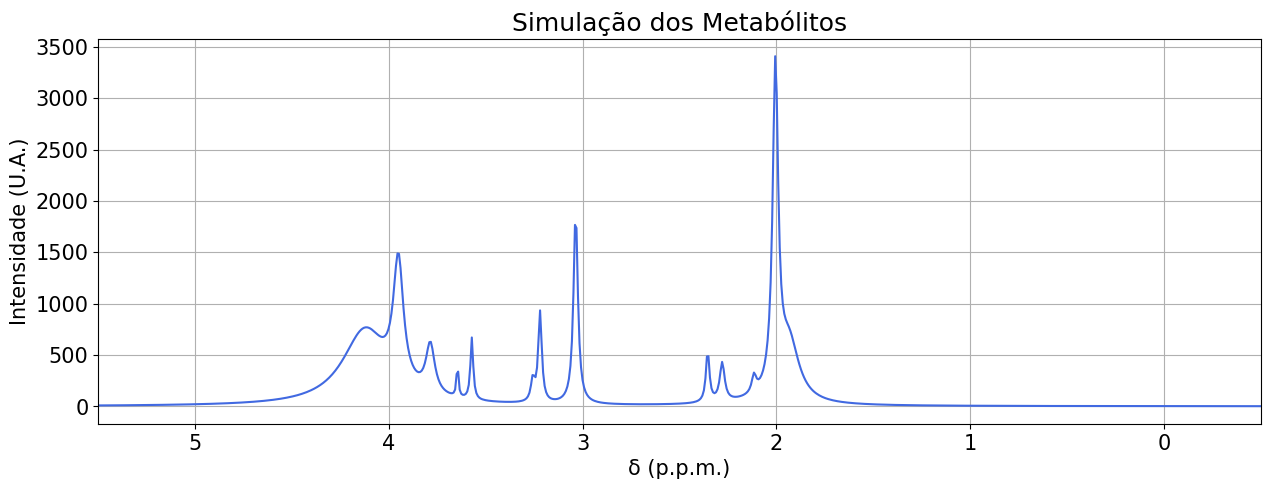
\includegraphics[scale=0.37]{metabolites.png}
    \caption{Resultado da simulação dos metabólitos}
    \label{fig:4}
\end{figure}

\subsection{Corrupção}

Apesar de o programa dar conta de simular espectros corretamente a partir dos parâmetros dados, a realidade é que sinais clínicos \textit{in vivo} tem uma aparência significativamente 
diferente da de um sinal gerado a partir do processo anteriormente descrito. 

Os métodos de aquisição e conversão de sinais analógicos em digitais, embora avançados se comparados à décadas passadas, ainda são limitados em várias instâncias. Uma das principais 
limitações ainda presentes é a captação de sinal ruidoso, o qual, a depender de sua intensidade, pode dificultar significativamente ou até impedir a análise do sinal desejado. A presença 
inevitável de ruído no sinal é, inclusive, uma das principais limitações as quais o MPM pretende enfrentar, tornando sua presença essencial neste estudo. 

\subsubsection{Geração}

No caso da maioria dos sinais captados, o ruído tem como distribuição geradora uma função gaussiana, definida pela equação \ref{eq:3}. Nessa distribuição, $\mu$ representa seu valor central, 
que no caso do ruído captado por aparelhos, tem valor nulo. O segundo parâmetro, $\sigma$, representa a largura do intervalo de variação dos valores gerados a partir dessa 
distribuição, definido como sendo o valor adquirido na meia altura da curva, denominado desvio padrão.


\begin{equation} \label{eq:3}
    f(x) = \frac{1}{\sigma \sqrt{2\pi}}e^{-\frac{(x - \mu)^2}{2\sigma ^2}}
\end{equation}

Essa distribuição, definida em um módulo de números aleatórios da biblioteca \textit{numpy}, foi usada para geração de um ruído complexo, de mesmo $\sigma$ na parte real e imaginária, que foi então adicionado ao sinal original, simulando assim sua
corrupção.

Para fins de controle adequado da corrupção do sinal, a Relação Sinal-Ruído (SNR) foi usada como métrica de sua qualidade. O cálculo da SNR não possui uma definição unificada, podendo variar significativamente a depender da área. Sendo assim, 
escolheu-se a que seria mais conveniente para o contexto apresentado, atentando-se também a qual seria mais comum nos trabalhos de referência desse projeto. A definição a ser usada é a que 
leva em consideração o pico do sinal e o desvio padrão do ruído \cite{}, como definido em \ref{eq:2}.  

\begin{equation} \label{eq:2}
    SNR = \frac{P}{\sigma}
\end{equation}

Para facilitar os cálculos, foi decidido normalizar o sinal gerado, dividindo-o pelo valor de seu pico, que se tornaria o valor de referência do sinal. O desvio padrão do ruído foi 
calculado então em uma região a qual esperaria-se que o sinal predominante seria de tal característica, que no caso dos metabólitos aqui simulados, se traduz na região final do sinal captado e do espectro.

\subsubsection{Relação entre desvios padrão}

Com o objetivo de obter maior controle da simulação, investigou-se o comportamento e a dependência entre o $\sigma$ utilizado para a geração de ruído na parte real e imaginária com o $\sigma$ resultante do espectro. A primeira abordagem 
tomada foi analítica, que a partir de definições estatísticas, não obteve sucesso na derivação de alguma relação direta. Optou-se então por uma abordagem experimental, a qual gerou-se um conjunto de sinais 
corrompidos por desvios padrão de diferentes valores, e relacionou-os com suas partes resultantes no espectro, calculados por meio de sua definição 
estatística em \ref{eq:5}.

\begin{equation} \label{eq:5}
    \sigma = \sqrt{\frac{1}{N} \sum_{i=1}^{N} (x_i - \bar{x})^2}, com \ \bar{x} = \frac{1}{N} \sum_{i = 1}^{N} x_i  
\end{equation}

Essa investigação possibilitaria a avaliação da implementação de uma função que, recebendo um valor desejado de SNR de entrada, forneceria qual deveria ser o valor aproximado do $\sigma$ usado pela distribuição 
geradora para que aquele valor de SNR fosse atingido, permitindo assim uma camada maior de controle dos parâmetros da simulação.



\section{Resultados e Discussão}

\begin{figure} [H]
    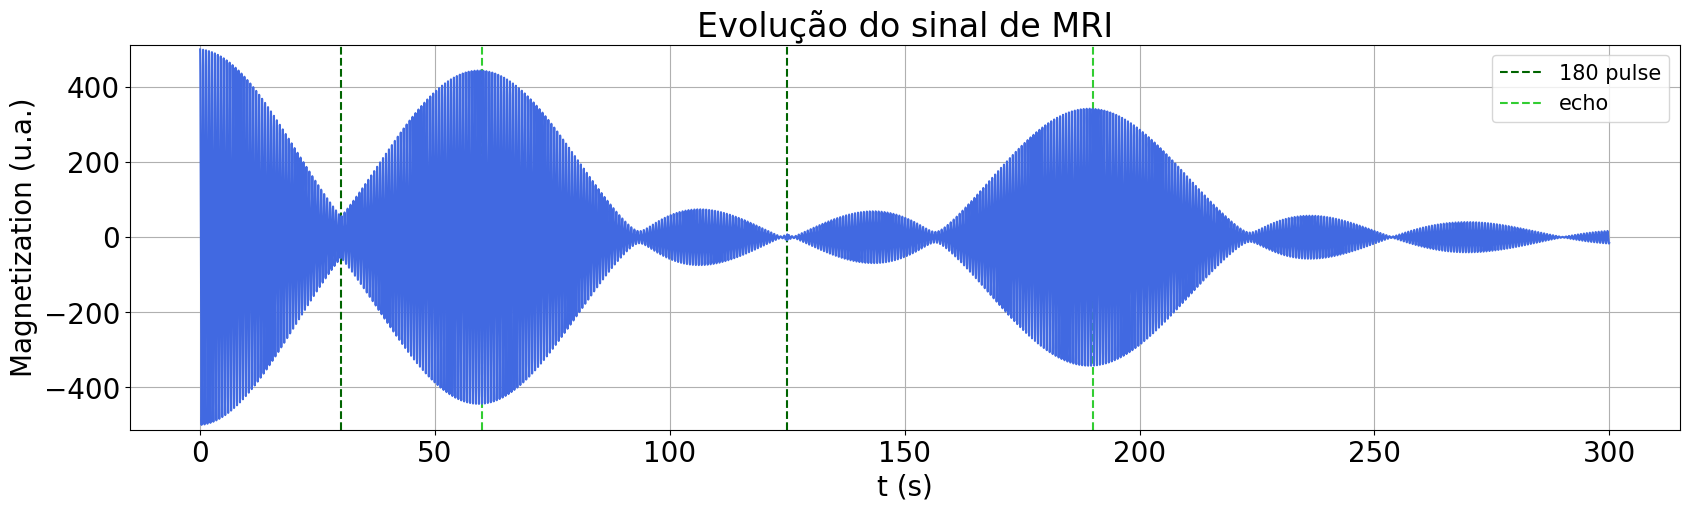
\includegraphics[scale=0.28]{spin-echo-example.png}
    \caption{Resultado da simulação de eco de spins}
    \label{fig:3}
\end{figure}

\begin{figure} [H]
    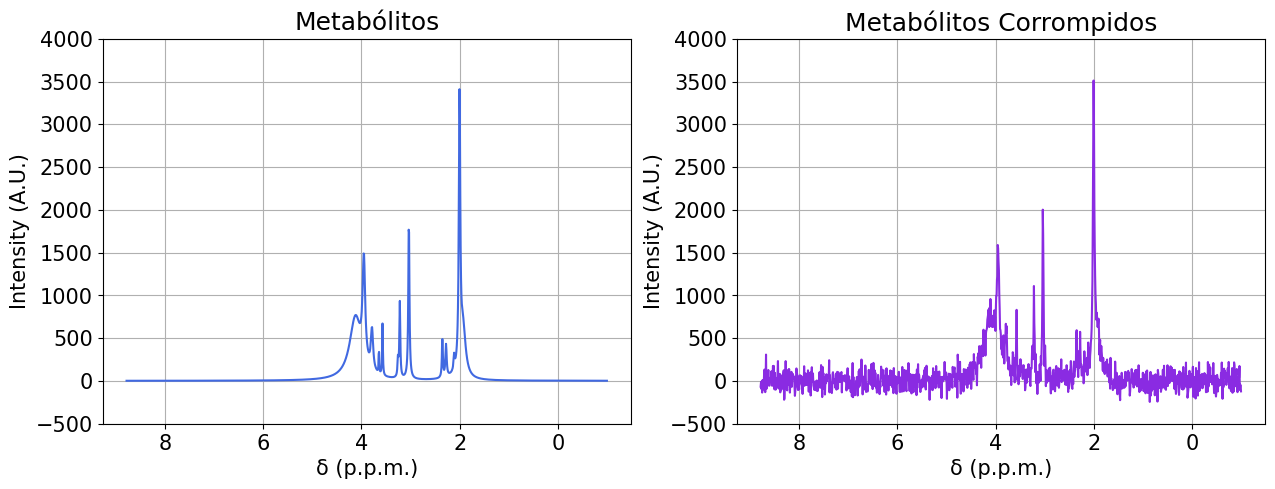
\includegraphics[scale=0.37]{metabolitos-corrompidos.png}
    \caption{Comparação entre os metabólitos e sua versão corrompida}
    \label{fig:5}
\end{figure}

\begin{figure} [H]
    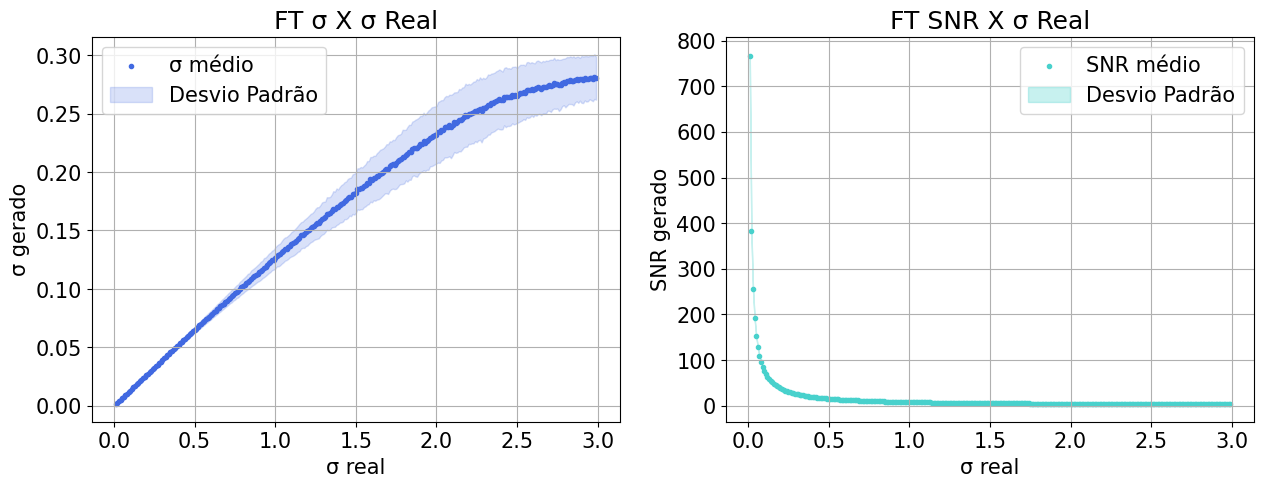
\includegraphics[scale=0.37]{evolucao-sigmas.png}
    \caption{Evolução do $\sigma$ gerado com relação ao $\sigma$ utilizado para a geração do ruído.}
    \label{fig:6}
\end{figure}

\begin{figure} [H]
    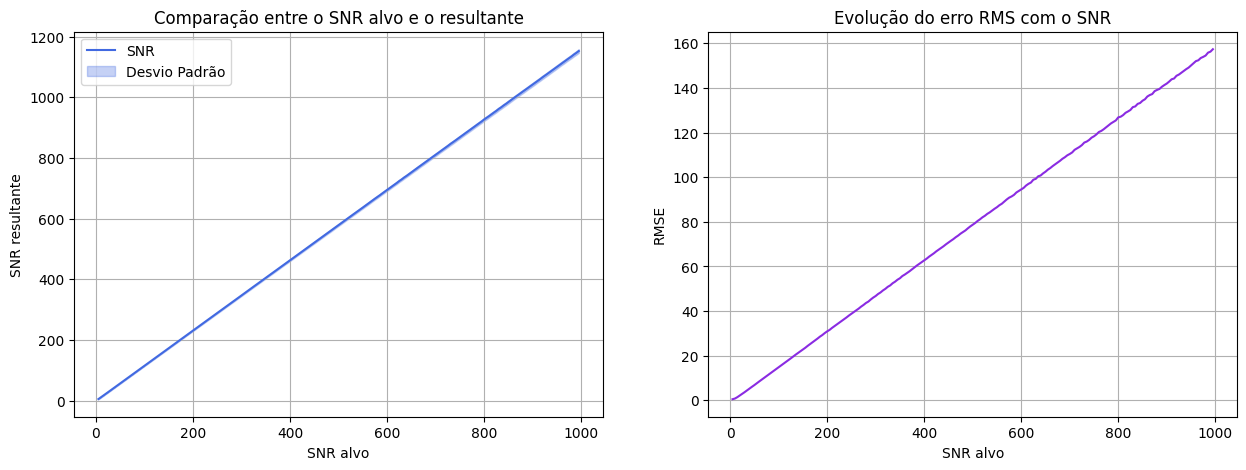
\includegraphics[scale=0.5]{evolucao-rmse-errado.png}
    \centering
    \caption{ERRADO Evolução do RMSE gerado com relação ao SNR requisitado.}
    \label{fig:7}
\end{figure}

\begin{figure} [H]
    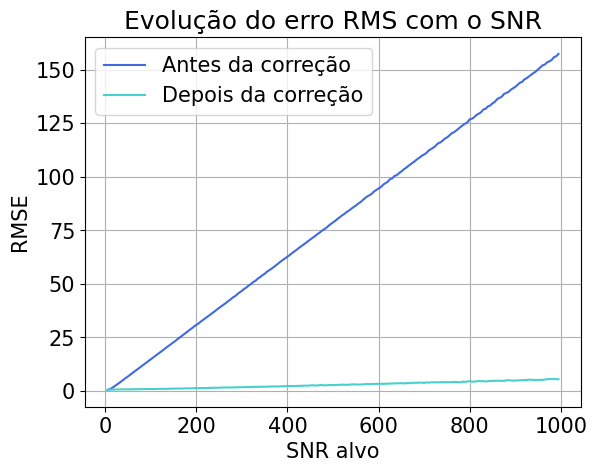
\includegraphics[scale=0.5]{evolucao-rmse.png}
    \centering
    \caption{Evolução do RMSE gerado com relação ao SNR requisitado após a correção.}
    \label{fig:8}
\end{figure}

\section{Conclusão}

A partir do estudo da relação entre desvios padrão e o SNR resultante, 
foi verificada uma relação linear para valores baixos de sigma, e uma 
saturação para valores mais altos. Também foram calculados 
parâmetros de ajuste dos dados, com os quais foi feita a correção dos 
valores de SNR de entrada, viabilizando a dedução de uma função que 
relacionasse diretamente sigma e SNR com uma margem de erro 
relativamente baixa para as intenções do projeto.


\bibliographystyle{plain}
\bibliography{refs}


%nding the document
\end{document}

%to compile, use pdflatex [name of the file].tex or use the compiler of vscode